\documentclass[conference]{IEEEtran}
% IEEE conference layout. Compile with pdfLaTeX.
% All diagrams and references are included in this file.
\usepackage{cite}
\usepackage{amsmath,amssymb}
\usepackage{graphicx}
\usepackage{booktabs}
\usepackage{tabularx}
\usepackage{url}
\usepackage{xcolor}
% Consistent result palette; marker shapes and line styles also identify series.
\definecolor{ResultBlue}{HTML}{0072B2}
\definecolor{ResultOrange}{HTML}{D55E00}
\definecolor{MatrixBlue}{HTML}{214E7C}
\usepackage{tikz}
\usetikzlibrary{arrows.meta,positioning}
\usepackage{pgfplots}
\pgfplotsset{compat=1.18}

\begin{document}
\title{Atomic Transfers and Fraud Review in a Concurrent Banking Prototype}
\author{
\IEEEauthorblockN{Harsh Bhatia, Tanisha Kapoor, Prakhar Garg}
\IEEEauthorblockA{Graphic Era (Deemed to be University)\\
Dehradun, India\\
24021741@geu.ac.in, 24022091@geu.ac.in, 240111564@geu.ac.in}}
\maketitle

\begin{abstract}
A transfer involves two balance changes, but the customer expects one outcome. This becomes harder to inspect when requests overlap, a payment is retried, or execution stops after a debit. We present a Python and SQLite banking prototype that exposes these cases through a web interface and a concurrency laboratory. Its payment service combines ordered account locks, explicit database transactions and persistent request keys. Evaluation comprised 45 automated tests and 24 short workloads with 2,400 operations. Every workload completed with the expected total balance and no negative account balance. Increasing the number of worker threads did not consistently reduce transfer-only completion time. A separate check of a saved BankSim classifier reproduced average precision of 0.6926, precision of 83.64 percent and recall of 51.52 percent on its original later-day test set. These results support the tested accounting behavior and an offline classification experiment. They do not establish real-bank detection accuracy. The prototype provides a practical way to examine where synchronization, persistence and payment review meet, and where their guarantees end.
\end{abstract}
\begin{IEEEkeywords}
banking prototype, transaction atomicity, thread synchronization,
SQLite, request replay, fraud review
\end{IEEEkeywords}

\section{Introduction}
Suppose an account contains INR 1,000 and two requests each try to withdraw INR 700. If both requests check the old balance, each can appear valid. A transfer adds another difficulty: a debit must not survive without its corresponding credit. Retrying a request after a delayed response creates a third case, since the first request may already have committed.

Our project makes these situations visible in a small banking application. Customers submit payments and inspect their history. An administrator reviews alerts and observes controlled concurrency demonstrations. Behind the interface, a shared Python service handles deposits, withdrawals and transfers against a SQLite database.

The work asks three questions:
\begin{enumerate}
\item Do the selected concurrency, retry and failure tests preserve the intended accounting properties?
\item How does completion time vary between one and twenty worker threads?
\item What can the available evidence establish about the fraud-review components?
\end{enumerate}
The contribution is an implemented teaching system with reproducible experiments and explicit component boundaries. It combines established mechanisms; it does not introduce a new concurrency-control algorithm.

Fraud review is included because a correct balance update does not determine whether a payment deserves investigation. We distinguish the website's deterministic rules, its optional external review, and a separately trained classifier. Their outputs answer different questions and require different forms of evaluation.

\section{Background and Related Work}
Berenson et al.~\cite{berenson} analyze ambiguities in SQL isolation definitions and the anomalies that different schedules can permit. Their treatment motivates checking concrete outcomes rather than treating the presence of a transaction statement as sufficient evidence of application correctness. Our tests examine balances, successful ledger entries and replay behavior.

SQLite describes a single-writer design and the use of \texttt{BEGIN IMMEDIATE} to start a write transaction before performing reads~\cite{sqlite}. Python's threading interface supplies locks, barriers and bounded acquisition waits~\cite{threading}. The prototype uses these at different levels: Python mutexes coordinate account operations within a process, while SQLite controls persistent updates.

Lopez-Rojas and Axelsson introduced BankSim as a simulator for generating payment data for fraud research~\cite{banksim}. It provides an experimental setting when private bank records are unavailable. Its synthetic origin does not establish that a classifier will transfer to another payment population. Saito and Rehmsmeier~\cite{saito} explain why precision-recall analysis is informative when positive cases are rare. We therefore report missed fraud cases alongside precision.

Unlike the cited isolation analysis or the BankSim simulator, this work evaluates a small end-to-end implementation. The purpose is to connect observable software behavior to its underlying mechanisms and document the limits of the evidence.

\section{System Design}
\subsection{Components and Data}
Fig.~\ref{fig:architecture} shows the implementation boundaries. Flask handles local HTTP requests, login state, customer/admin roles, account ownership and form tokens. The trusted command-line tool and simulator call the transaction service directly. They do not provide the website's authentication boundary.

\begin{figure}[t]
\centering
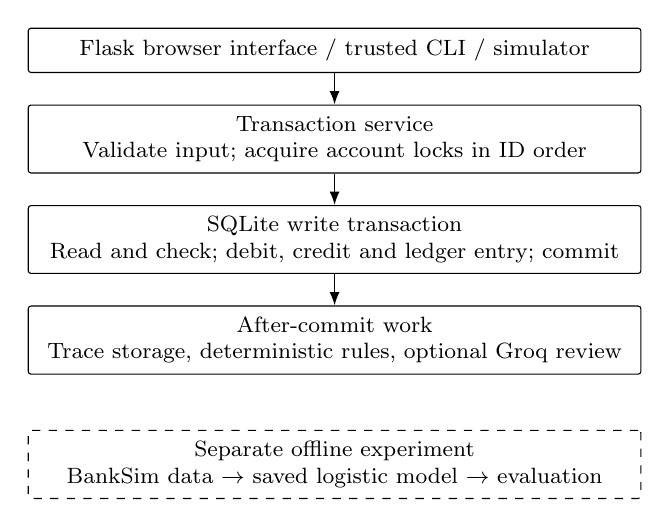
\begin{tikzpicture}[
 node distance=4mm,
 box/.style={draw,rounded corners=1pt,align=center,
 text width=7.5cm,inner sep=4pt,font=\footnotesize},
 flow/.style={-{Latex[length=1.7mm]},semithick}]
\node[box] (entry) {Flask browser interface / trusted CLI / simulator};
\node[box,below=of entry] (service) {Transaction service\\
Validate input; acquire account locks in ID order};
\node[box,below=of service] (db) {SQLite write transaction\\
Read and check; debit, credit and ledger entry; commit};
\node[box,below=of db] (review) {After-commit work\\
Trace storage, deterministic rules, optional Groq review};
\node[box,below=7mm of review,dashed] (offline) {Separate offline experiment\\
BankSim data $\rightarrow$ saved logistic model $\rightarrow$ evaluation};
\draw[flow] (entry)--(service);
\draw[flow] (service)--(db);
\draw[flow] (db)--(review);
\end{tikzpicture}
\caption{Execution boundaries. The offline model does not score live transfers. After-commit records have a separate persistence boundary from the payment.}
\label{fig:architecture}
\end{figure}

The database links users to accounts and records successful operations in a transaction ledger. Each success has a unique request key. Separate tables store failed attempts, fraud alerts, login attempts and execution events. Schema checks restrict operation types, source/destination combinations and nonnegative balances.

Amounts are integer paise, allowing whole-number arithmetic. Every operation opens its own connection. Initialization enables write-ahead logging (WAL); connections enable foreign keys and use \texttt{synchronous=FULL}. These settings describe the implementation, not a completed crash-recovery evaluation.

\subsection{Payment Protocol}
A transfer follows this sequence:
\begin{enumerate}
\item Validate the amount, account identifiers and request key.
\item Acquire relevant account mutexes in ascending ID order.
\item Open a connection and execute \texttt{BEGIN IMMEDIATE}.
\item Check for a committed operation with the same key. Return its result if the request matches; reject conflicting reuse.
\item Read current account state, check status and funds, update both balances, and insert the successful ledger row.
\item Commit, close the connection and release the locks.
\end{enumerate}
An error in the database transaction triggers rollback. The test interface can deliberately raise an error after the source debit, allowing the rollback path to be inspected. Eligible failed attempts are audited afterward in a different transaction. Malformed input rejected before execution is not recorded by this audit path.

The request key distinguishes a retry from a new payment. Reusing a committed key with the same operation returns the earlier transaction identifier. A failed request has no committed success row and can be retried. This defines replay behavior without claiming exactly-once delivery over a network.

\subsection{Lock Ordering and Its Limits}
Manager instances share an account-lock registry keyed by the resolved database path. A thread acquiring locks in ascending order cannot hold a higher-ID account lock while waiting for a lower-ID one. A cycle formed only from these ordered account locks therefore cannot arise.

This reasoning does not imply fairness or starvation freedom. The account-lock acquisition budget and SQLite's busy wait are separate; the whole operation is not bounded by one lock timeout. A failure audit can require a further database wait.

The registry exists only within one Python process. Separate processes rely on database transaction control for persistent writes. The evaluation includes independent registries in different threads, but does not claim a full multiprocess deployment test. Account mutexes do not turn SQLite into a database with concurrent row-level writers.

\subsection{Tracing and Review}
Web receipts expose observed lock and database events. Successful payment traces are saved after commit. The laboratory uses temporary databases and controlled race/deadlock examples, so those exercises do not alter customer demonstration balances.

Rules flag conditions such as a transfer of at least INR 5,000 or five outgoing transfers within sixty seconds. Additional rules inspect failed operations, unsuccessful logins and unauthorized account access. These thresholds are demonstration settings.

When configured, Groq receives limited transfer context and returns a concern category with an explanation. Tests use controlled responses rather than live-provider calls. An unavailable review service does not undo the payment; the saved BankSim model is not a fallback. Traces and reviews are separate writes, so a payment may exist without all supporting records if a later write fails.

\section{Evaluation Method}
\subsection{Accounting Properties}
Let $b_i$ be an account balance, $D$ the sum of successful deposits and $W$ the sum of successful withdrawals. For a workload without unrelated concurrent activity, the expected total is
\begin{equation}
\sum_i b_i^{\mathrm{final}} =
\sum_i b_i^{\mathrm{initial}} + D - W.
\label{eq:accounting}
\end{equation}
Internal transfers contribute neither to $D$ nor to $W$. The simulator also checks $b_i^{\mathrm{final}}\geq0$, worker completion and whether every submitted operation has a success or rejection outcome.

A final total alone cannot prove that each account received the correct amount. Individual tests therefore inspect specific balances, ledger rows and request results. Table~\ref{tab:tests} summarizes selected assertions.

\begin{table}[t]
\caption{Selected Assertions from the Passing Test Suite}
\label{tab:tests}
\centering\footnotesize
\begin{tabularx}{\columnwidth}{@{}p{0.26\columnwidth}X@{}}
\toprule
Scenario & Expected outcome checked by the test\\
\midrule
Concurrent deposits & 100 deposits of INR 100 increase INR 10,000 to INR 20,000; 100 ledger rows.\\
Competing withdrawals & Of 20 requests for INR 1,000, ten succeed against INR 10,000; closing balance zero.\\
Injected failure & Error after debit leaves both balances unchanged and no committed payment row.\\
Duplicate key & Twenty concurrent requests with one key produce one new payment.\\
Opposing transfers & Two threads perform 25 transfers each in opposite directions; starting balances are restored.\\
Independent registries & Forty concurrent deposits through separate registries preserve the expected total.\\
Web boundaries & Ownership, roles, form tokens, receipts, alert rules and mocked review failures are checked.\\
\bottomrule
\end{tabularx}
\end{table}

\subsection{Repeated Workloads}
The experiments recorded on 2 November 2026 used a fresh temporary database for each run. Three accounts began with INR 10,000 each. A queue held 100 requests. Transfer mode sampled two distinct accounts and an integer amount from INR 1 to INR 100. Mixed mode also selected deposit, withdrawal or transfer with equal probability.

Both modes ran with 1, 5, 10 and 20 workers, three times per configuration, producing 24 runs. Seed 42 fixed request generation; seed 2026 shuffled configuration order. Repeating a seed fixes requests, not operating-system scheduling.

The timer included thread creation, barrier synchronization and worker completion. Database initialization, seeding and queue construction were outside the timer. Runs invoked the service without web tracing or external review calls.

The recorded environment was Python 3.12.14, SQLite 3.53.1 and Windows 11 build 26200. The processor identifier was Intel64 Family 6 Model 142 Stepping 12. Background load, power state and filesystem cache were not controlled. Sample standard deviation and mean per-run throughput are descriptive; three repetitions do not provide a strong statistical performance guarantee.

\section{Transaction Results}
All 45 automated tests passed in 121.108 seconds. All 24 workloads satisfied the balance, nonnegativity and completion checks. Across them, 2,400 operations succeeded, with no rejections, unexpected errors or failure-audit warnings. Amounts were small relative to starting balances. Rejection under insufficient funds was exercised separately by the withdrawal test.

Table~\ref{tab:timings} reports the timings. Throughput is the mean of three individual run rates, so it need not equal 100 divided by the mean completion time. Fig.~\ref{fig:timing} shows completion-time variation, while Fig.~\ref{fig:throughput} compares the number of operations completed per second. Both plots use the same recorded workloads.

\begin{table}[t]
\caption{Completion Time for 100 Operations; Three Runs per Row}
\label{tab:timings}
\centering\footnotesize
\begin{tabular}{@{}lrrrr@{}}
\toprule
Mode & Threads & Mean (s) & SD (s) & Mean ops/s\\
\midrule
Transfer & 1 & 3.865 & 0.365 & 26.02\\
Transfer & 5 & 4.004 & 0.793 & 25.62\\
Transfer & 10 & 3.673 & 0.732 & 28.03\\
Transfer & 20 & 3.794 & 0.720 & 27.07\\
Mixed & 1 & 3.823 & 1.252 & 28.02\\
Mixed & 5 & 3.108 & 0.270 & 32.33\\
Mixed & 10 & 3.218 & 0.758 & 32.42\\
Mixed & 20 & 2.524 & 0.351 & 40.12\\
\bottomrule
\end{tabular}
\end{table}

\begin{figure}[t]
\centering
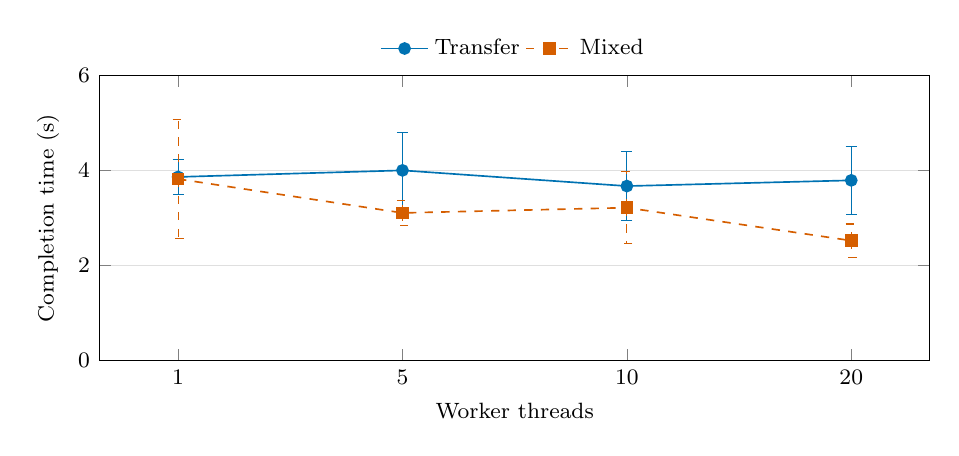
\begin{tikzpicture}
\begin{axis}[
 width=\columnwidth,height=5.2cm,
 xlabel={Worker threads},ylabel={Completion time (s)},
 xmin=0.65,xmax=4.35,ymin=0,ymax=6,
 xtick={1,2,3,4},xticklabels={1,5,10,20},
 tick label style={font=\footnotesize},
 label style={font=\footnotesize},
 legend style={font=\footnotesize,at={(0.5,1.02)},anchor=south,legend columns=2,draw=none},
 ymajorgrids=true,grid style={gray!25}]
\addplot+[color=ResultBlue,semithick,mark=*,
 mark options={solid,fill=ResultBlue,draw=ResultBlue},
 error bars/.cd,y dir=both,y explicit]
coordinates {
(1,3.8655) +- (0,0.3648)
(2,4.0038) +- (0,0.7925)
(3,3.6733) +- (0,0.7320)
(4,3.7938) +- (0,0.7200)};
\addlegendentry{Transfer}
\addplot+[color=ResultOrange,semithick,dashed,mark=square*,
 mark options={solid,fill=ResultOrange,draw=ResultOrange},
 error bars/.cd,y dir=both,y explicit]
coordinates {
(1,3.8226) +- (0,1.2519)
(2,3.1079) +- (0,0.2703)
(3,3.2180) +- (0,0.7584)
(4,2.5238) +- (0,0.3508)};
\addlegendentry{Mixed}
\end{axis}
\end{tikzpicture}
\caption{Mean time with one sample standard deviation. Worker counts are equally spaced categories. Error bars are not confidence intervals.}
\label{fig:timing}
\end{figure}

\begin{figure}[tb]
\centering
% Means and sample SDs computed from the three recorded per-run rates.
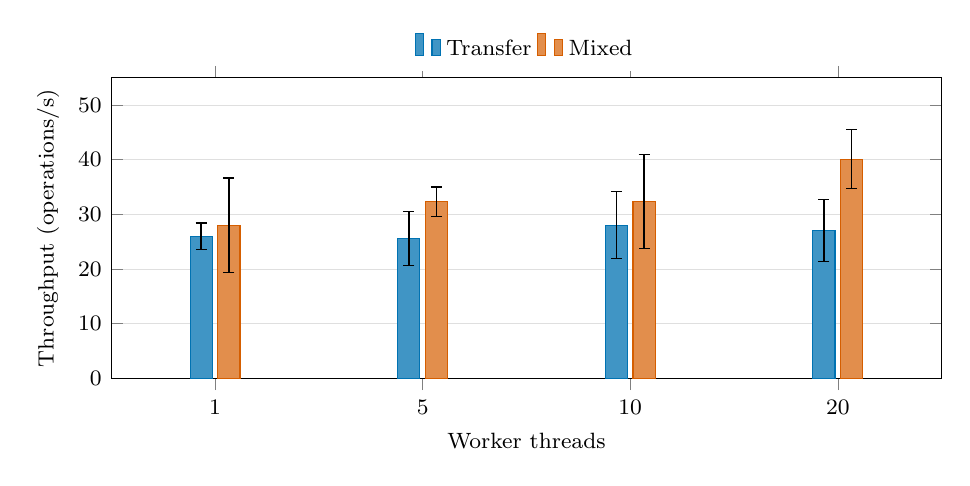
\begin{tikzpicture}
\begin{axis}[
 width=\columnwidth,height=5.4cm,
 ybar,bar width=8pt,
 xlabel={Worker threads},ylabel={Throughput (operations/s)},
 xmin=0.5,xmax=4.5,ymin=0,ymax=55,
 xtick={1,2,3,4},xticklabels={1,5,10,20},
 ytick={0,10,20,30,40,50},
 tick label style={font=\footnotesize},
 label style={font=\footnotesize},
 legend style={font=\footnotesize,at={(0.5,1.02)},anchor=south,legend columns=2,draw=none},
 ymajorgrids=true,grid style={gray!25},
 error bars/error bar style={black,semithick}]
\addplot+[draw=ResultBlue,fill=ResultBlue!75,
 error bars/.cd,y dir=both,y explicit]
coordinates {
(1,26.0200) +- (0,2.4132)
(2,25.6233) +- (0,4.9321)
(3,28.0333) +- (0,6.1175)
(4,27.0733) +- (0,5.6551)};
\addlegendentry{Transfer}
\addplot+[draw=ResultOrange,fill=ResultOrange!70,
 error bars/.cd,y dir=both,y explicit]
coordinates {
(1,28.0200) +- (0,8.6473)
(2,32.3333) +- (0,2.6900)
(3,32.4200) +- (0,8.5940)
(4,40.1167) +- (0,5.3550)};
\addlegendentry{Mixed}
\end{axis}
\end{tikzpicture}
\caption{Mean throughput for 100-operation workloads, with one sample standard deviation across three runs per configuration. All submitted operations succeeded. The bars summarize this local experiment; they do not establish a general scalability result.}
\label{fig:throughput}
\end{figure}

Transfer-only means ranged from 3.67 to 4.00 seconds. They do not show a consistent reduction as worker count increases. The mixed workload had a lower mean at twenty workers than at one, but its intermediate results were not monotonic. These measurements do not isolate scheduling, connection setup or disk activity as the cause.

The throughput view gives the same conclusion in operational terms: transfer-only means stayed between 25.62 and 28.03 operations/s. Mixed workloads reached 40.12 operations/s at twenty workers in this sample. The error bars show that the mean alone does not describe the variation between runs; with only three repetitions, they should not be read as confidence intervals.

Only three accounts are involved, and SQLite allows one writer at a time~\cite{sqlite}. Additional threads therefore need not create additional simultaneous updates. No comparison with account mutexes removed was performed, so a speed advantage from that layer cannot be inferred. The supported result is preservation of the tested accounting rules.

\section{Offline Fraud-Model Evaluation}
\subsection{Data and Training}
The local BankSim CSV contains 594,643 labelled records. Its source address and SHA-256 are recorded with the saved model. The training script builds three features before updating customer history: $\log(1+a)$ for amount $a$, earlier payments by the same customer on that day capped at twenty, and an indicator that the customer--merchant pair has not appeared before.

The split uses the 80th percentile of the day field as the cutoff. It assigns 472,365 earlier-day rows to training and 122,278 later-day rows to testing; the test period begins at step 147. There are 5,880 fraud labels in training and 1,320 in testing. A standard scaler is fitted only to training rows. Logistic regression uses a maximum of 1,000 iterations and random state 42.

\subsection{Verification of the Saved Model}
The stored coefficients were applied again to their original test period; the model was not retrained. A scan confirmed nondecreasing day steps in CSV order and matched the data hash to the training artifact. Historical features still follow file order within each day; finer event chronology was not established.

Re-scoring reproduced precision and recall exactly, with average precision differing from the saved value by less than $10^{-12}$. This is a reproducibility check on an existing holdout, not an independent validation dataset.

\begin{table}[t]
\caption{Saved Model Re-evaluated on Its Original BankSim Holdout}
\label{tab:model}
\centering\footnotesize
\begin{tabular}{@{}lr@{}}
\toprule
Measure & Result\\
\midrule
Test rows & 122,278\\
Fraud-labelled rows & 1,320\\
Average precision & 0.6926\\
Precision at threshold 0.5 & 83.64\%\\
Recall at threshold 0.5 & 51.52\%\\
True positives / false positives & 680 / 133\\
False negatives / true negatives & 640 / 120,825\\
\bottomrule
\end{tabular}
\end{table}

\subsection{Interpretation}
Table~\ref{tab:model} includes successful detections and errors. About 1.08\% of the test rows are labelled fraud. Predicting every row as legitimate would already achieve about 98.92\% accuracy, making accuracy alone unhelpful here. Average precision combines precision values over increases in recall~\cite{ap}; it is distinct from precision at the chosen threshold.

At threshold 0.5, the classifier identified 680 fraud-labelled payments but missed 640. Of its 813 flagged payments, 133 were false positives. Fig.~\ref{fig:confusion} displays these outcomes alongside the correctly classified legitimate payments. Each percentage uses the actual class total as its denominator, so the large legitimate class does not hide the missed fraud cases. This offers a concrete discussion of missed cases and review workload. It does not demonstrate that the prototype prevents fraud.

\begin{figure}[tb]
\centering
% Rows: actual class. Columns: predicted class. Shade = row percentage.
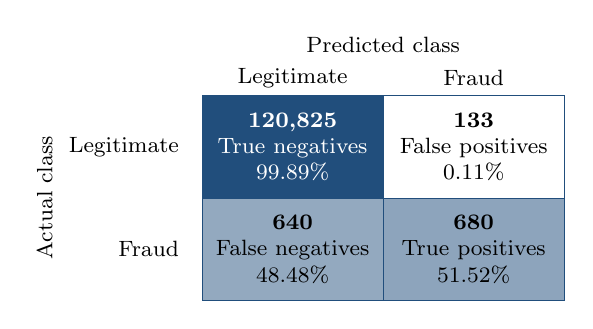
\begin{tikzpicture}[x=1cm,y=1cm,font=\footnotesize]
\node at (4.0,3.25) {Predicted class};
\node at (2.85,2.83) {Legitimate};
\node at (5.15,2.83) {Fraud};
\node[rotate=90] at (-0.30,1.30) {Actual class};
\node[anchor=east,align=right] at (1.53,1.95) {Legitimate};
\node[anchor=east,align=right] at (1.53,0.65) {Fraud};
\filldraw[fill=MatrixBlue!99.89,draw=MatrixBlue] (1.7,1.3) rectangle (4.0,2.6);
\filldraw[fill=MatrixBlue!0.11,draw=MatrixBlue] (4.0,1.3) rectangle (6.3,2.6);
\filldraw[fill=MatrixBlue!48.48,draw=MatrixBlue] (1.7,0) rectangle (4.0,1.3);
\filldraw[fill=MatrixBlue!51.52,draw=MatrixBlue] (4.0,0) rectangle (6.3,1.3);
\node[align=center,text=white] at (2.85,1.95)
 {\textbf{120,825}\\True negatives\\99.89\%};
\node[align=center] at (5.15,1.95)
 {\textbf{133}\\False positives\\0.11\%};
\node[align=center] at (2.85,0.65)
 {\textbf{640}\\False negatives\\48.48\%};
\node[align=center] at (5.15,0.65)
 {\textbf{680}\\True positives\\51.52\%};
\end{tikzpicture}
\caption{Confusion matrix for the saved BankSim model at threshold 0.5 on its original 122,278-row holdout. Counts are shown with percentages within each actual-class row; darker blue indicates a larger row percentage. The rows contain 120,958 legitimate and 1,320 fraud-labelled payments. These are offline results.}
\label{fig:confusion}
\end{figure}

The model's amount distribution and simulated-day activity feature have not been calibrated for INR transfers and the application's rolling time windows. It remains outside the live website path. Rule tests verify selected triggers; mocked Groq tests verify integration behavior. Neither establishes accuracy on actual customer payments. No live-provider latency or detection experiment is reported.

\section{Discussion and Limitations}
The accounting tests answer the first research question for the executions observed. An injected partial debit is rolled back, and repeated committed request keys do not cause a second payment. These checks support the chosen transaction boundary; the total-balance invariant adds a workload-level check.

The second question has a narrower answer: additional threads did not consistently improve transfer-only time. Three repetitions, short queues and three shared accounts are insufficient for a general scalability conclusion. A stronger comparison would vary account population, request mix and seeds, measure individual latency percentiles, and include database-only synchronization as a baseline.

For the third question, evidence must stay attached to the component tested. The classifier was evaluated on synthetic BankSim rows. Website rules were tested against selected conditions. External-review behavior was tested with mocks. Combining these into one fraud-accuracy claim would hide their different meanings.

There are further limits:
\begin{itemize}
\item \emph{Concurrency coverage:} finite tests do not explore every schedule. Independent registries were exercised in threads, not separate processes. Ordered account locks do not establish fairness.
\item \emph{Failure coverage:} an injected exception is not a process kill, power loss or storage fault. Recovery, backup restoration and failover were not measured.
\item \emph{Supporting records:} alerts, traces and failure audits are separate writes. Reliable delivery needs further design if every committed payment must have those records.
\item \emph{Timing validity:} experiments used one Windows machine without controlled background load. Network and browser latency are excluded.
\item \emph{Detection validity:} the saved model and holdout were reused. No new threshold selection, probability calibration or real-payment validation was performed.
\end{itemize}

The deliberate lost-update and circular-wait demonstrations also need careful interpretation. They force conditions using barriers and dummy locks. They show why a mechanism matters; they do not estimate how often that failure occurs in a deployed bank.

\section{Conclusion}
The prototype gives students a payment path they can inspect from validation to persistent balance changes and later review records. In the recorded evaluation, 45 automated tests passed and 24 workloads completed 2,400 operations with the expected accounting totals. Timing results did not justify a claim that more threads make transfers faster. Re-evaluating the saved BankSim model reproduced its metrics and exposed substantial missed detections at the chosen threshold. Broader concurrency and crash testing, reliable review-record delivery, and validation on suitable independent payment data are the next steps.

\section*{Reproducibility}
Measurements were recorded on 2 November 2026. Core source hashes still matched that evaluated snapshot when this manuscript was prepared. Companion evidence includes \path{evaluation_results.json} and \path{model_evaluation.json}, containing raw runs, environment details and source hashes.

In the project workspace, \path{docs/research/evaluate.py} repeats temporary-database workloads. The adjacent \path{evaluate_model.py} re-scores saved parameters and requires the local BankSim CSV. Tests run with \texttt{python -m unittest discover -s tests -v}. Repository:
\url{https://github.com/harshbhatia04/secure-banking-system}.
At manuscript preparation, the new research files were local additions; evidence is supplied separately rather than assumed to be in the public repository.

\section*{Acknowledgment}
The authors thank their project mentor, Prof. Dr. Mohammad Wazid, for his guidance and feedback during the development of this project.

\begin{thebibliography}{00}
\bibitem{berenson}
H. Berenson, P. Bernstein, J. Gray, J. Melton, E. O'Neil, and P. O'Neil,
\lq\lq A critique of ANSI SQL isolation levels,\rq\rq\
in \emph{Proc. ACM SIGMOD}, 1995, pp. 1--10.
[Online]. Available:
\url{https://www.microsoft.com/en-us/research/wp-content/uploads/2016/02/tr-95-51.pdf}

\bibitem{sqlite}
SQLite, \lq\lq Isolation in SQLite.\rq\rq\
Accessed: Nov. 2, 2026. [Online]. Available:
\url{https://www.sqlite.org/isolation.html}

\bibitem{threading}
Python Software Foundation, \lq\lq threading---Thread-based parallelism,\rq\rq\
\emph{Python 3.12 Documentation}. Accessed: Nov. 2, 2026.
[Online]. Available: \url{https://docs.python.org/3.12/library/threading.html}

\bibitem{banksim}
E. A. Lopez-Rojas and S. Axelsson,
\lq\lq BankSim: A bank payments simulator for fraud detection research,\rq\rq\
in \emph{Proc. 26th European Modeling and Simulation Symposium},
2014, pp. 144--152. [Online]. Available:
\url{https://www.msc-les.org/proceedings/emss/2014/EMSS2014_144.pdf}

\bibitem{saito}
T. Saito and M. Rehmsmeier,
\lq\lq The precision-recall plot is more informative than the ROC plot when
evaluating binary classifiers on imbalanced datasets,\rq\rq\
\emph{PLOS ONE}, vol. 10, no. 3, Art. no. e0118432, 2015,
doi: 10.1371/journal.pone.0118432.

\bibitem{ap}
scikit-learn developers, \lq\lq average\_precision\_score,\rq\rq\
\emph{API Reference}. Accessed: Nov. 2, 2026. [Online]. Available:
\url{https://scikit-learn.org/stable/modules/generated/sklearn.metrics.average_precision_score.html}
\end{thebibliography}
\end{document}
